% ***********************************************************
% ******************* PHYSICS HEADER ************************
% ***********************************************************
% Version 2
\documentclass[11pt]{article} 
\usepackage{amsmath} % AMS Math Package
\usepackage{amsthm} % Theorem Formatting
\usepackage{amssymb}	% Math symbols such as \mathbb
\usepackage{graphicx} % Allows for eps images
\usepackage{multicol} % Allows for multiple columns
\usepackage[dvips,letterpaper,margin=0.75in,bottom=0.5in]{geometry}
 % Sets margins and page size
\pagestyle{empty} % Removes page numbers
\makeatletter % Need for anything that contains an @ command 
\renewcommand{\maketitle} % Redefine maketitle to conserve space
{ \begingroup \vskip 10pt \begin{center} \large {\bf \@title}
	\vskip 10pt \large \@author \hskip 20pt \@date \end{center}
  \vskip 10pt \endgroup \setcounter{footnote}{0} }
\makeatother % End of region containing @ commands
\renewcommand{\labelenumi}{(\alph{enumi})} % Use letters for enumerate
% \DeclareMathOperator{\Sample}{Sample}
\let\vaccent=\v % rename builtin command \v{} to \vaccent{}
\renewcommand{\v}[1]{\ensuremath{\mathbf{#1}}} % for vectors
\newcommand{\gv}[1]{\ensuremath{\mbox{\boldmath$ #1 $}}} 
% for vectors of Greek letters
\newcommand{\uv}[1]{\ensuremath{\mathbf{\hat{#1}}}} % for unit vector
\newcommand{\abs}[1]{\left| #1 \right|} % for absolute value
\newcommand{\avg}[1]{\left< #1 \right>} % for average
\let\underdot=\d % rename builtin command \d{} to \underdot{}
\renewcommand{\d}[2]{\frac{d #1}{d #2}} % for derivatives
\newcommand{\dd}[2]{\frac{d^2 #1}{d #2^2}} % for double derivatives
\newcommand{\pd}[2]{\frac{\partial #1}{\partial #2}} 
% for partial derivatives
\newcommand{\pdd}[2]{\frac{\partial^2 #1}{\partial #2^2}} 
% for double partial derivatives
\newcommand{\pdc}[3]{\left( \frac{\partial #1}{\partial #2}
 \right)_{#3}} % for thermodynamic partial derivatives
\newcommand{\ket}[1]{\left| #1 \right>} % for Dirac bras
\newcommand{\bra}[1]{\left< #1 \right|} % for Dirac kets
\newcommand{\braket}[2]{\left< #1 \vphantom{#2} \right|
 \left. #2 \vphantom{#1} \right>} % for Dirac brackets
\newcommand{\matrixel}[3]{\left< #1 \vphantom{#2#3} \right|
 #2 \left| #3 \vphantom{#1#2} \right>} % for Dirac matrix elements
\newcommand{\grad}[1]{\gv{\nabla} #1} % for gradient
\let\divsymb=\div % rename builtin command \div to \divsymb
\renewcommand{\div}[1]{\gv{\nabla} \cdot #1} % for divergence
\newcommand{\curl}[1]{\gv{\nabla} \times #1} % for curl
\let\baraccent=\= % rename builtin command \= to \baraccent
\renewcommand{\=}[1]{\stackrel{#1}{=}} % for putting numbers above =
\newtheorem{prop}{Proposition}
\newtheorem{thm}{Theorem}[section]
\newtheorem{lem}[thm]{Lemma}
\theoremstyle{definition}
\newtheorem{dfn}{Definition}
\theoremstyle{remark}
\newtheorem*{rmk}{Remark}

% ***********************************************************
% ********************** END HEADER *************************
% ***********************************************************
\usepackage{cancel}
\usepackage{verbatim}
\usepackage{graphicx}
\newcommand{\Le}{\left}
\newcommand{\Ri}{\right}
\usepackage{enumerate}
\usepackage{appendix}
\title{Comp 350 assignment 6}
\author{Ian Benlolo 260744397\\McGill University \\}
\begin{document}
\maketitle
\begin{enumerate}[1.]
%%question 1
\item
	\begin{enumerate}[(a)]
	\item
\textbf{Trapezoid}
$$\left|I-I_R\right|= \left|\frac{-1}{12}(b-a)h^2f''(z)\Ri| $$ where $h=\frac{b-a}{n}$\\
$$\Le| \frac{-1}{12}\frac{(b-a)^3}{n^2}f''(z)\Ri|=\Le|\frac{-1}{12}\frac{(1-0)^3}{n^2}f''(z) \Ri| = \frac{1}{12n^2}\Le|f''(z)\Ri|,\ we\ want\  \frac{1}{12n^2}max_{\in [0,1]} \Le| f''(z)\Ri| \leq 10^{-6}$$
$$f(x)=\frac{2}{\sqrt{\pi}}e^{-z^2}, \ f'(z)=\frac{2}{\sqrt{\pi}}(-ze^{-2z^2})$$ $$f''(z)=\frac{2}{\sqrt{\pi}}(-2e^{-z^2}+4z^2e^{-z^2})=\frac{2}{\sqrt{\pi}}e^{-z^2}(4z^2-2)$$ $$f'''(z)=\frac{2}{\sqrt\pi}[4ze^{-z^2}+8ze^{-z^3}-8z^3e^{-z^3}]=\frac{8}{\sqrt\pi}ze^{-z^2}(3-2z^2)=0 $$ So either $z=0$ or $3-2z^2=0\rightarrow 2z^2=3,\ z=\pm\sqrt{\frac{3}{2}}$. The latter is ignored since $\pm\sqrt{\frac{3}{2}}$ are out of the $[0,1]$ range\\
Now,\\
$$\frac{1}{12n^2}\times max\{f\Le|f''(0)\Ri|, \Le|f''(1)\Ri| \} \leq 10^{-6},$$where, $\Le|f''(0)\Ri|=\Le| \frac{2}{\sqrt\pi}\times-2\Ri|=\Le|\frac{-4}{\sqrt\pi}\Ri| =\frac{4}{\sqrt\pi}$ and $f''(1)=\frac{2}{e\sqrt\pi}(4-2)=\frac{4}{e\sqrt\pi}$. So $f''(0)$ is the bigger of the two.\\
$$\frac{1}{12n^2}\frac{4}{\sqrt\pi}\leq10^{-6}\rightarrow n^2\geq \frac{1}{3\sqrt\pi}10^6\Rightarrow n\geq \sqrt{\frac{1}{3\sqrt\pi}10^6} \approx 434$$


	\item\item Here are the results of my programs and the code
		
	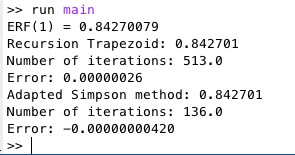
\includegraphics{results.jpg}
	\begin{verbatim}
	function [result, y] = RecursionTrapezoid(a, b)
  %setting h to b-a, and x is the first step
h = b-a;
x = h/2*(f(0)+f(1));
count=2;
m = 0;
%if the difference between the actual erf(1) and x is
%greater than 10^-6 then recursively do the trapezoid computation
while abs(erf(1)-x) > 10^(-6)
    h = h/2;
    m = m+1;
    sum = 0;
    for i=1:2^(m-1)
        sum = sum + f(a+(2*i-1)*h);
        count = count + 1;
    end
    x = h*sum + x/2;
end
result = x;
y = count;
end

----------------------------------------------------------------------------------------
function soln = adapt_simpson(a,b,ep,lvl, lvl_max, count)
h = b-a;
c = (a+b)/2;
i1=h*(f(a)+4*f(c)+f(b))/6;
count = count + 3;
lvl = lvl + 1;
d=(a+c)/2;
e=(c+b)/2;
i2 = h*(f(a)+4*f(d)+2*f(c)+4*f(e)+f(b))/12;
count = count + 5;
if lvl >= lvl_max
    numbI = i2;
    soln = [numbI, count];
else
    if abs(i2-i1) <= 15*ep
        numbI = i2+(1/15)*(i2-i1);
        soln = [numbI, count];
    else
       soln = adapt_simpson(a,c,ep/2,lvl, lvl_max, count) 
       		+ adapt_simpson(c,b,ep/2,lvl, lvl_max, count); # put on a different 
                                                     # line to fit the margins
    end
end
end\end{verbatim}

	\end{enumerate}
	
	
	%%quesiton 2
	\item
	We want $I_G=\alpha f(-\frac{1}{2})+\beta f(0)+\gamma f(-\frac{1}{2})$. $A_0=\alpha,\ A_1=\beta\ A_2=\gamma$ \& $x_0=-\frac{1}{2},\ x_1=0,\ x_2=\frac{1}{2}$.\\
	$$A_0=\int_{-1}^1\frac{(x-0)(x-\frac{1}{2})}{(-\frac{1}{2}-0)(-\frac{1}{2}-\frac{1}{2})}dx = 2\int_{-1}^{1}x^2-\frac{1}{2}xdx=2\Le[\frac{x^3}{3}-\frac{x^2}{4}\Ri]_{-1}^1=\dots=\frac{4}{3}$$
	$$A_1=\int_{-1}^1\frac{(x+\frac{1}{2})(x-\frac{1}{2})}{(0+\frac{1}{2})(0-\frac{1}{2})}dx=-4\int_{-1}^1x^2-\frac{1}{4}dx=-4\Le[\frac{x^3}{3}-\frac{x}{4}\Ri]_{-1}^1=\dots=-\frac{2}{3}$$
	$$A_2=\int_{-1}^1\frac{(x-0)(x+\frac{1}{2})}{(\frac{1}{2}-0)(\frac{1}{2}+\frac{1}{2})}dx=2\int_{-1}{1}x^2+\frac{x}{2}dx=\dots=\frac{4}{3}$$
	Therefore
	$$I_G=\frac{4}{3}f(-\frac{1}{2})-\frac{2}{3}f(0)+\frac{4}{3}f(\frac{1}{2})$$
\end{enumerate}
\end{document}